%===========================================
% Smart Metering Uncertainty Forecasting
%
% Author  Estevao "Steve" Alvarenga
%         efsa@bath.edu
% Created in 10/Jun/17
%-------------------------------------------
% smuf_ovlf Publication
%===========================================

%===========================================
% Setup, Packages
%===========================================

%% Copyright 2009 Elsevier Ltd
%%
%% This file is part of the 'Elsarticle Bundle'.
%% ---------------------------------------------
%%
%% It may be distributed under the conditions of the LaTeX Project Public
%% License, either version 1.2 of this license or (at your option) any
%% later version.  The latest version of this license is in
%%    http://www.latex-project.org/lppl.txt
%% and version 1.2 or later is part of all distributions of LaTeX
%% version 1999/12/01 or later.
%%
%% Template article for Elsevier's document class `elsarticle'
%% with numbered style bibliographic references
%%
%% $Id: elsarticle-template-1-num.tex 149 2009-10-08 05:01:15Z rishi $
%% $URL: http://lenova.river-valley.com/svn/elsbst/trunk/elsarticle-template-1-num.tex $
%%
\documentclass[preprint,3p,12pt,authoryear]{elsarticle}

%% Use the option review to obtain double line spacing
%% \documentclass[preprint,review,12pt]{elsarticle}

%% Use the options 1p,twocolumn; 3p; 3p,twocolumn; 5p; or 5p,twocolumn
%% for a journal layout:
%% \documentclass[final,1p,times]{elsarticle}
%% \documentclass[final,1p,times,twocolumn]{elsarticle}
%% \documentclass[final,3p,times]{elsarticle}
%% \documentclass[final,3p,times,twocolumn]{elsarticle}
%% \documentclass[final,5p,times]{elsarticle}
%% \documentclass[final,5p,times,twocolumn]{elsarticle}

%% The graphicx package provides the includegraphics command.
\usepackage{graphicx}
%% The amssymb package provides various useful mathematical symbols
\usepackage{amssymb}
%% The amsthm package provides extended theorem environments
\usepackage{amsthm}
%% Allowing my name to be written
\usepackage[utf8]{inputenc}
%% Enhanced math expressions
\usepackage{amsmath}
\usepackage{bm}
\usepackage{color,soul}
\usepackage[noadjust]{cite}
%% Nice tables
\usepackage{booktabs}


%% The lineno packages adds line numbers. Start line numbering with
%% \begin{linenumbers}, end it with \end{linenumbers}. Or switch it on
%% for the whole article with \linenumbers after \end{frontmatter}.
\usepackage{lineno}

%% natbib.sty is loaded by default. However, natbib options can be
%% provided with \biboptions{...} command. Following options are
%% valid:
%%   round  -  round parentheses are used (default)
%%   square -  square brackets are used   [option]
%%   curly  -  curly braces are used      {option}
%%   angle  -  angle brackets are used    <option>
%%   semicolon  -  multiple citations separated by semi-colon
%%   colon  - same as semicolon, an earlier confusion
%%   comma  -  separated by comma
%%   numbers-  selects numerical citations
%%   super  -  numerical citations as superscripts
%%   sort   -  sorts multiple citations according to order in ref. list
%%   sort&compress   -  like sort, but also compresses numerical citations
%%   compress - compresses without sorting
%%
\biboptions{comma,round}

\graphicspath{{graphics/}{graphics/arch/}{Graphics/}{./}} % Look in these folders for graphics


%===========================================
% Article
%===========================================

\journal{International Journal of Forecasting}

\begin{document}

\begin{frontmatter}

%% Title, authors and addresses

\title{Forecast-based Portfolio Optimisation of Electricity Demand for Peer to Peer Markets}
%\title{Smart Meter Uncertainty Forecast}
%-------------------------------------------
% Contribution
% 1- APPL: local balancing, from national to distribution level, p2p mkt, reduced total energy cost, minimise generation loss, etc
% 2- TECH: old tech invalid because of uncertainty level, new tech: portfolio optim
%-------------------------------------------

%% use the tnoteref command within \title for footnotes;
%% use the tnotetext command for the associated footnote;
%% use the fnref command within \author or \address for footnotes;
%% use the fntext command for the associated footnote;
%% use the corref command within \author for corresponding author footnotes;
%% use the cortext command for the associated footnote;
%% use the ead command for the email address,
%% and the form \ead[url] for the home page:
%%
%% \title{Title\tnoteref{label1}}
%% \tnotetext[label1]{}
\author{Estêvão Ferreira Sêco de Alvarenga\corref{cor1}\fnref{label2}}
% \ead{efsa@bath.edu}
% \ead[url]{home page}
\author{Jooyoung Jeon\fnref{label2}}
\author{Ran Li\fnref{label3}}
\author{Fotios Petropoulos\fnref{label2}}
\author{Furong Li\fnref{label3}}
\address{University of Bath, UK\fnref{label3}}
\cortext[cor1]{efsa@bath.edu}
\fntext[label2]{University of Bath School of Management}
\fntext[label3]{University of Bath Department of Electronic \& Electrical Engineering}

%% use optional labels to link authors explicitly to addresses:
%% \author[label1,label2]{<author name>}
%% \address[label1]{<address>}
%% \address[label2]{<address>}

\begin{abstract}
We propose to produce probabilistic forecasts for a group of households rather than individual households to minimise forecast uncertainty in Peer to Peer (P2P) trading, which aims to utilise surplus in renewable energy generation locally.
% To produce the probabilistic forecasts, we used two probabilistic forecast models: Kernel density estimation (KDE) and ARMA-GARCH. (better define ARMA-GARCH and KDE on forecasting methods)
Our study compares the characteristics of the Irish and Korean smart meter data we used, and finds that probabilistic forecast accuracy enhances with a larger aggregation of customers, and converges to the maximum in average for groups larger than 50 customers, which is recommended as the number of minimum customers in a P2P transaction when the aggregation is constructed in a random manner. Aiming to produce a better probabilistic forecast accuracy conditional on an expected supply, the research further explores three approaches to defining an aggregation of customers, and finds that the approach simply using standard deviation only in the in-sample period produces probabilistic forecasts comparable to or better than more sophisticated approaches. Our empirical analysis uses hourly data from Korea and Ireland to evaluate the density forecasts of group demand up to 24h ahead.
% Check Irish data/result is included. Any further findings?
\end{abstract}

\begin{keyword}
Science \sep Publication \sep Complicated
%% keywords here, in the form: keyword \sep keyword
%% MSC codes here, in the form: \MSC code \sep code
%% or \MSC[2008] code \sep code (2000 is the default)
\end{keyword}


\end{frontmatter}

%% Start line numbering here if you want
\linenumbers

%===========================================
\section{Introduction}
\label{sec:intro}
%===========================================
As the world drives towards increased renewable energy adoption, a greater proportion of generation is coming from local sources.
These distributed energy resources (DER) are mainly based on technologies such as medium to small solar arrays, locally generated waste, and wind sources, and have increased alongside other modern energy solutions like batteries, small-scale hydro, tides and electric vehicles (EV). The DER could feed local distribution networks and sell excess capacity into the grid \citep {HAIN20051199}.
Nevertheless, most of them are not actively utilised by the distribution network or electricity retailers due to the negative impact on network stability and the lack of incentives from an active local energy marketplace.
This has simplified their participation in the market as load reduction assets, with low penetration level.

To maximise the utilisation of DER, \citet{pouttu2017p2p} propose a smart electricity business model based on peer-to-peer (P2P) trading.
This framework is currently used to enable decentralised business transactions across several industries, such as investment, labour, goods and transport.
Companies such as eBay and Airbnb connect thousands of buyers and a sellers, allowing experimentation with prices and different selling mechanisms \citep{p2p_mkts}.

\citet{pouttu2017p2p} suggest the P2P philosophy is well suited and even preferred when a large number of DER are connected to the grid, enabling them to embrace more strategic opportunities towards active roles in the power market.

Additionally, DER can act as groups, and trade services within organised energy market auctions, such as frequency response, peak-shaving or spare capacity usage \citep{energycollectives2017preprint}.
These services, based on aggregating load and/or generation from several DER, are overseen by a new legal actor in the energy market: the Aggregator.
To be able to effectively trade at the power system market, the Aggregator will need support from a bespoke platform.
This platform must be able to look at high frequency individual demand data and monitor, predict, schedule and assess risk regarding energy trading in real time \citep{mocanu2016demand}.



This paper analyses the relationship between expected aggregated demand and density forecast errors.
We relate them, respectively, to 'return' and 'risk' from the classical portfolio theory, as illustrated in Figure \ref{fig:random_frontier}.

\begin{figure}
  \centering
  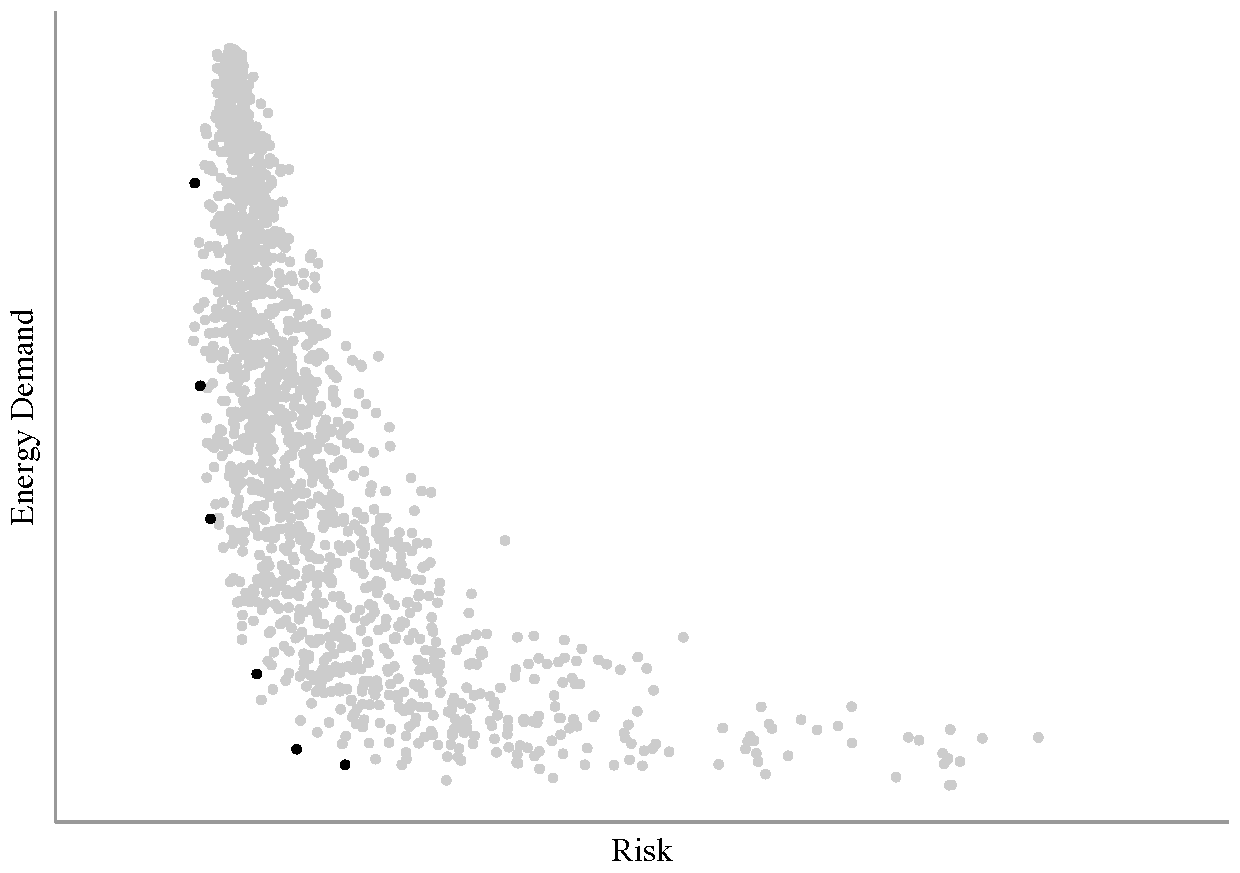
\includegraphics[width=0.8\columnwidth]{2018-01-03_randomgrouping_frontier}
  \caption{The expected demand for a forecast-based portfolio of customers and its risk measured as the forecast error. Various random aggregations are shown in light grey, while the preferred values that minimises risk are in the frontier built by dark points.}
  \label{fig:random_frontier}
\end{figure}

Forecast errors (risk) are defined through a time-series based forecast function that couples historical demand volume and load variation data with recent development on probabilistic forecast and computer power.
One advantage of using time series data is the simplicity and flexibility for implementing the same model in other regions or using other type of customers.
It also does not depend on weather or socio-economical data availability, as it uses past trend and behaviour for extrapolating the future energy requirement \citep{forecasting_general_review}.
Having said that, wherever there is additional datasets available, regression based models could be used to enhance accuracy.
This have been proved to enhance the prediction accuracy in noisy financial time series forecasting \citep{TAY2001309}.
Expected aggregated demand (return) is defined by past data.

Based on portfolio optimisation of density forecasts, the paper compares various customers selection methods.
The goal is to propose a method that choses a portfolio with minimal forecast errors for a given energy demand.
The methods we propose can help Aggregators match demand in an uncertainty scenario with surplus in local generation.

\hl{The rest of the paper is organised as follows: ...}

%===========================================
\section{The Korean smart meter data}
\label{sec:smdata}
%===========================================

The Korean data consists of hourly demand of 1,000 residential customers, recorded between January 2012 and October 2014 by Korea Electric Power Corporation (KEPCO).
None of the data sources contains specific location data.
To avoid some periods of missing observations, we did not use the first 12 weeks of data, which contained too many empty data points.
For missing observations in the in-sample data, the value of the same hour of the same day of the previous week was used instead, to maintain the daily and weekly seasonal patterns.
We did not evaluate the performance of our models in the missing period in the out-of-sample.

Figure \ref{fig:4weeks} illustrates different patterns of demand time series in the same four week period for four different customers in February 2012.
Cycles of 24h and 168h (one week) are present in the data.

\begin{figure}
  \centering
  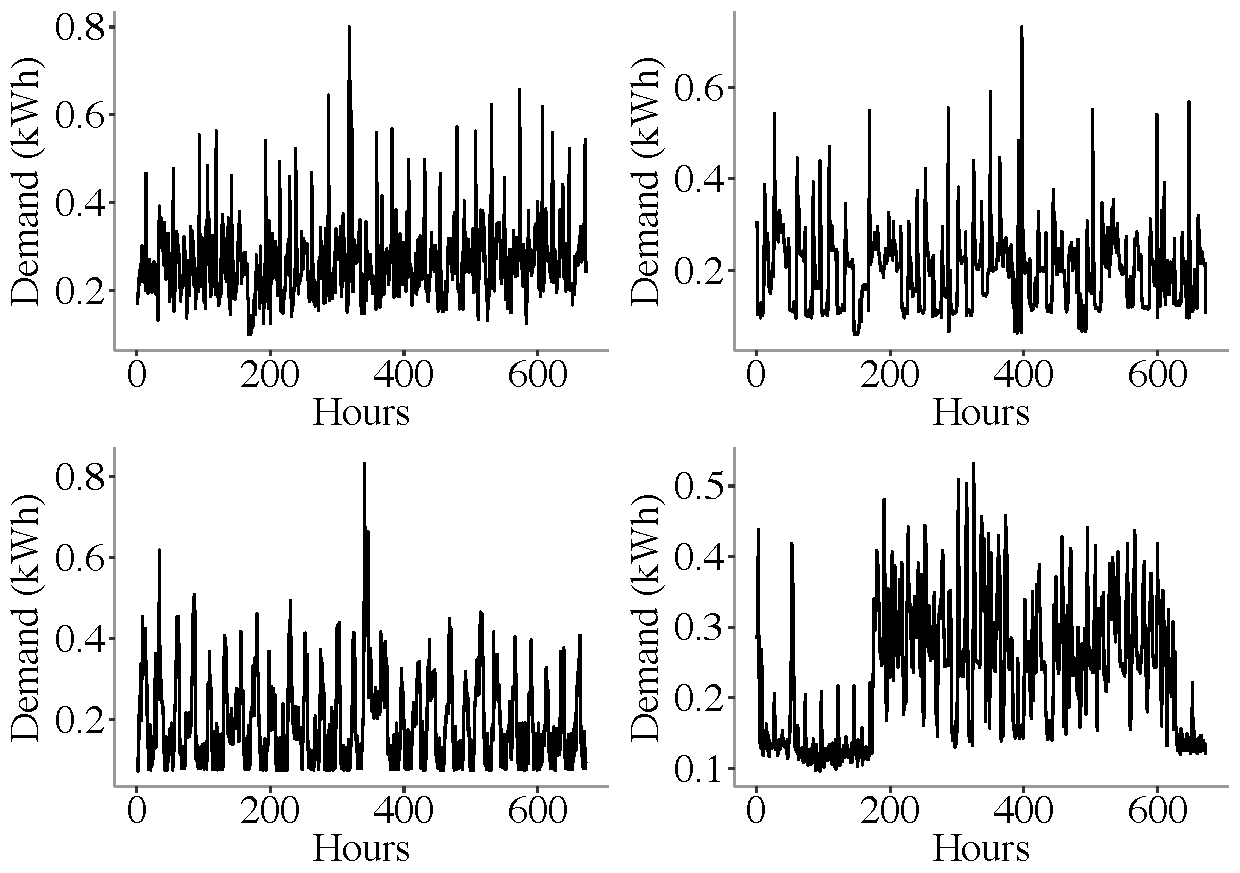
\includegraphics[width=0.8\columnwidth]{2017-10-13_compare_demands_bw2}
  \caption{Example of electricity demand pattern for four different customers during a period of four weeks[WHICH MONTH/YEAR AND WHICH COUNTRY DATA?]}
  \label{fig:4weeks}
\end{figure}

Datasets containing 12 weeks were used for model fitting and forecast generation for up to the next 72 hours.
We had access to a a very big high frequency dataset.
Instead of using a rolling forecast approach, for each possible hour of available data, we summarised the data as follows:
For the initial analysis on models and parameters, before any forecast results for the paper were collected, we used forecasting starting points 37 hours apart of each other.
This allowed for the forecasts to start in different hours inside weeks.
For data collected for results and discussion, we used sections of the dataset 113 hours apart of each other.
This method would enable us to use data from several years for the initial analysis without disrupting the blindness of the datasets for forecasting.
Also, it allowed us to research a big space of the original dataset, and not have a high bias toward certain week days or times of day, while restricting computational time to a feasible cost.

%===========================================
\section{Density forecasting for energy demand}
\label{sec:load_fcst}
%===========================================
Generally, medium- and long-term forecasts must take into account the historical load and weather data, the number of customers in different categories, the appliances in the area and their characteristics including age, the economic and demographic data and their forecasts, the appliance sales data, and other factors \citep{feinberg2005load}.
This longer forecasts are used to predict loads as distant as twenty years ahead, so that expansion planning can be facilitated.
Large generation and infrastructure projects depend on this kind of forecasting for supporting decision \citep{soliman1997application}.

Short-term electric load forecasting, on the other hand, is vital for power generation and operation.
It is fundamental in many applications such as providing optimal economic generation, system security, and management and planning \citep{Hamadi200447}.
It can also be used to capture value via intra-day or intra-week power arbitrage (moving energy from low value periods to high value periods).

Short to medium-term forecasting models have to take account the relationship between demand and weather.
However, for lead times of 1-day-ahead there is little difference between performance compared to not using forecasted weather data.
Non-weather models accuracy worsen as lead time increases, being dominated by more complex models \citep{TAYLOR200357}.

When the interest is in lead times up to about six hours ahead, a univariate model is deemed to be sufficient.
Whenever the availability of weather forecasts is patchy, univariate models are used for lead times larger than six hours ahead \citep{TAYLOR20061}.
In the short run, the load is mainly influenced by meteorological real time conditions, seasonal effects (daily and weekly cycles, calendar holidays) and special events.

While the decision making process in the utility industry rely on expected values, or point forecasting, the increase in market competition and renewable integration requires a probabilistic approach for planning and operation of energy systems \citep{HONG2016914}.
Literature provides a wide range of electricity demand forecasting methods, with probabilistic approaches being favoured due to non-linear and non-stationary demand profiles \citet{mocanu2016demand}.
The research interest in probabilistic energy forecasting has taken off rapidly in recent years \citep{Hong2016896} and, at the same time, a massive smart meter deployment providing the industry a huge amount of high resolution data \citep{HONG2016914}.

%-------------------------------------------
\subsection{Seasonal analysis}
\label{ss:dtransf}
%-------------------------------------------
Energy demand has natural cycles and the forecasting method we selected (described on Section \ref{ss:fcst}) is not expected to produce good forecasts unless data has no trend.
While some  methods can handle seasonality, whenever the chosen one can not, it is considered a good strategy to analyse seasonal components, and remove them from the data, before running forecasts.

The oldest approach to handling seasonality in time series is to extract it using a seasonal decomposition procedure such as the X-11 method.
In addition to work on the X-11 method and its variants, there have also been several new methods for seasonal adjustment developed, the nonparametric method STL being one of them \citep{DEGOOIJER2006443}.

STL (seasonal-trend decomposition based on Loess) addresses the main drawbacks from X-11, without letting go of its innovations.
X-11 has a complex option selection procedure, is difficult to diagnose, and is not prepared to deal with missing data.
The more recent STL method does not suffer from these, while delivering a robust seasonal and trend-cycle decomposition that is not distorted by transient, aberrant behaviour in the data \citep{cleveland1990stl}.
On the other hand, STL is limited to addictive decomposition, unless some form of data-transformation is implemented to obtain multiplicative decompositions.

STL is a filtering procedure for decomposing the original data $Y_t$ into trend-cycle $T_t$, seasonal $S_t$ and residual $R_t$ (\ref{eq:stl1}), using a local regression technique known as Loess.

\begin{equation}
   Y_t = T_t + S_t + R_t
   \label{eq:stl1}
\end{equation}

Loess delivers distance-weighted least-squares fit, of polynomials of degree $d$, to localised subsets of $q$ elements from the data containing $n$ elements.
Large $q$ results in traditional smoother regressions, while $q\to\infty$ generates ordinary polynomial fits.
STL consists on two procedures, updating seasonal and trend components, while computing robustness weights recursively.
We implemented the STL seasonal analysis as the first step of our procedure.
This was done using the R \texttt{\textbf{stats}} package \citep{r}.

%-------------------------------------------
\subsection{Forecasting procedure}
\label{ss:fcst}
%-------------------------------------------
In this Section, we describe the forecasting procedure implemented.
According to \citet{TAYLOR200357} there is no consensus as to the best approach to electricity demand forecasting.
In this paper we implement an univariate autoregressive conditional heteroskedasticity (ARMA-GARCH) model supported by an unconditional kernel density estimation (KDE) model.

For each customer, in each time-step, we define an ARMA-GARCH model to produce forecasts, as described on Section \ref{sss:arma-garch}.
Whenever this model does not converge to an acceptable fit, we implement the KDE model, described on Section \ref{sss:kde}.
The acceptable fit is defined via the adjusted Pearson chi-squared goodness-of-fit test, proposed by \citet{vlaarpalm_gof}.
Section \ref{sss:gof.min} details the implementation and results for the dataset used on this paper.

Finally, on Section \ref{sss:eval} we introduce the continuous ranked probability score (CRPS), the evaluation criteria of choice for the produced density forecasts.

%-------------------------------------------
\subsubsection{Kernel density estimation}
\label{sss:kde}
%-------------------------------------------

Kernel density estimation (KDE) is a non-parametric method.
This means it can maintain the original properties, avoiding any previous assumptions of distributions, constructing the density function based on historic observations.
Similar to the unconditional KDE implementation done by \citet{Arora201647}, \citet{Jeon2016991} and \citet{Taylor2015370}, the method enables the non-parametric estimation of a probability density \(f\) based on observations \(\{Y_{1},Y_{2},...,Y_{n}\}\).
The unconditional KDE can be defined through Equation \ref{eq:kde}:

\begin{equation}
   \hat f(y) = \sum_{w=1}^{W} K_{h_y} (Y_W - y) %efsa 2do check this formula
   \label{eq:kde}
\end{equation}

where $y$ is the energy demand forecast to be estimated, $W$ is the size of the sliding window $w$, i.e. number of observations, and $K$ is a Gaussian kernel function with bandwidth $h_y$.

The bandwidth is responsible for the density smoothness and was chosen according to Silverman’s reference bandwidth, also known as Silverman’s rule of thumb \citep{silverman1986density}.
This method defines the bandwidth through Equation \ref{eq:kde.bw}:

\begin{equation}
   h = \begin{cases}
      0.9 \hat \sigma n^{-\frac{1}{5}}\ , & \text{if $\hat \sigma<\frac{sIQR}{1.34}$}\ , \\
      0.9 \frac{sIQR}{1.34} n^{-\frac{1}{5}}\ , & \text{otherwise}.
    \end{cases}
   \label{eq:kde.bw}
\end{equation}

where $\hat \sigma$ is the standard deviation of the sliding window $w$ and $sIQR$ is the sample interquartile range.

Figure \ref{fig:dens.cus} exemplifies density plots for the same 24 hours for different customers using Korean data.
\begin{figure}
  \centering
  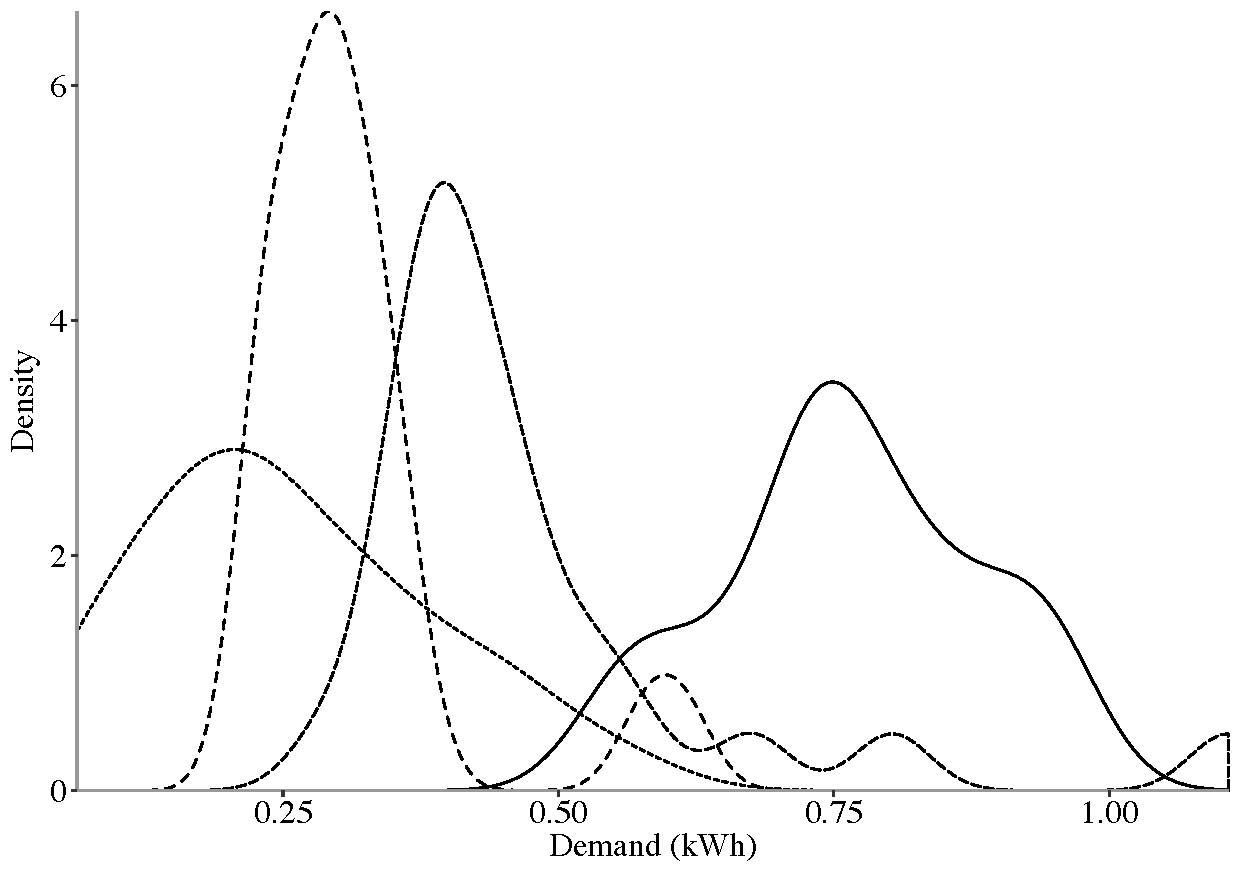
\includegraphics[width=0.8\columnwidth]{2017-10-13_compare_fulldensities_KO2}
  \caption{Example of electricity demand densities forecasted for four different individual customers, built using KDE with a window size of 24h, without prior seasonal analysis}
  \label{fig:dens.cus}
\end{figure}

%-------------------------------------------
\subsubsection{Univariate ARMA-GARCH}
\label{sss:arma-garch}
%-------------------------------------------

According to \citet{Jeon2016991}, ARMA-GARCH models are used widely for capturing autocorrelation in the conditional mean and variance.
GARCH models were used to predict day-ahead electricity prices in Spain and California, outperforming general time series ARIMA models, specially when high volatility is present \citep{garcia2005garch}.
The ARMA($r,m$) describes the conditional mean process, while the GARCH($p,q$) describes the conditional variance process.
The GARCH($p,q$) process is similar to an ARMA process implemented for the variance magnitude.
The ARMA($r,m$)-GARCH($p,q$) model follows Equations \ref{eqsub:arma} to \ref{eqsub:error}.
[YOU USED s for seasonality]
\begin{subequations}
   \begin{align}
      y_t        & = \alpha_0 + \sum_{j=1}^p \alpha_j Y_{t-j} + \sum_{k=1}^q \beta_k \varepsilon_{t-k}
         \label{eqsub:arma} \\
      \sigma^2_t & = \delta_0 + \sum_{l=1}^r \delta_j \sigma^2_{t-l} + \sum_{m=1}^s \gamma_k \varepsilon^2_{t-m}
         \label{eqsub:garch}\\
      \varepsilon_t & = \sigma_t \eta_t
         \label{eqsub:error}
   \end{align}
   \label{eq:arma_garch}
\end{subequations}

where $y_t$ is the energy demand observed at time $t$;
$\epsilon_t$ is a iid error term;
$\sigma_t$ is the conditional standard deviation (volatility);
$\alpha_i$, $\beta_i$, $\delta_i$ and $\gamma_i$ are the coefficients of the AR, MA, GARCH and ARCH components with orders defined by non-negative integers $p$, $q$, $r$ and $s$, respectively;
and $\eta_t$ is the white noise generating process.
In principle the $\varepsilon_t$ could follow any suitable distribution model.

We used the R package \texttt{\textbf{rugarch}} to build the ARMA-GARCH model \citep{Ghalanos_2014}.
The ARMA($r,m$) order was defined via the lowest Bayesian Information Criterion (BIC) value for the combination of possible ($p,q$) up to ($5,5$).
BIC was described by \citet{schwarz1978} as an evaluation criteria for choosing the appropriate dimensionality of a model.
The main difference between BIC and maximum likelihood or Akaike Information Criteria (AIC) is the application of a higher penalty for high order models.
We chose to limit ($p,q$) up to ($5,5$) as we deemed this was a good trade-off between forecast accuracy and computing resources.
The GARCH($p,q$) order was set to (1,1) as this has been shown to produce accurate practical result for volatility estimation \citep{hansen2001comparison}.

For the distribution selection, \texttt{\textbf{rugarch}} enables the use of normal, student-t, generalised error distribution and their skewed versions.
\citet{theodossiou2015skewed} investigated empirical distributions for finance data with the presence of skewness, kurtosis, conditional heteroskedasticity, asymmetric volatility, and other non-linear dependencies.
This properties created biased models when applying normal distributions.
A skewed version of the generalised error distribution was proven to provide better fit to the empirical distribution of the data. Based on this, and to accommodate a highly volatile dataset, we chose this distribution for the ARMA-GARCH model.

%-------------------------------------------
\subsubsection{Evaluation criteria}
\label{sss:eval}
%-------------------------------------------
With the forecasts in hands, we accordingly added back the deterministic seasonality removed previously, as described in Section \ref{ss:dtransf}.
The trend-cycle component was extrapolated with the last value recorded in the in-sample data and added to the forecasts.
We then used the continuous ranked probability score (CRPS) for the evaluation of uncertainty forecasts.

The method, described in \citet{GBR2007crps}, assesses probabilistic forecasts of continuous variables that take the form of predictive densities or cumulative distributions.
The CRPS generalises the absolute error, to which it reduces in case of point forecasts, and assess probabilistic forecasts against deterministic observations.
The CRPS is reported in the same unit as the observations.

The formal definition of this scoring method is described in Equation \ref{eq:crps}.

\begin{equation}
   \text{CRPS} = \int_{-\infty}^{\infty} \text{BS}(y) dy
   \label{eq:crps}
\end{equation}

Where BS denotes the Brier Score \citep{brier1950verification} of probability forecasts, as in Equation \ref{eq:bs}.

\begin{equation}
   \text{BS} = \frac{1}{N} \sum_{i=1}^N {(p_i - o_i)}^2
   \label{eq:bs}
\end{equation}

Where $p_i$ is the density forecast and $o_i$ is the observed value.

The goal is the maximisation of the sharpness of the predictive distributions subject to calibration.
While calibration refers to the statistical consistency between the predictive distributions and observations, sharpness is a forecast property that refers to the concentration of the predictive distributions.

%-------------------------------------------
\subsubsection{Fit convergence for ARMA-GARCH models}
\label{sss:gof.min}
%-------------------------------------------
\hl{include figure with arma garch not fitting from presentation}
Since the optimisation needed for Section \ref{ss:portopt} depends on a calibrated forecast function, this section describes how the fit convergence for ARMA-GARCH models were defined.
This parameter is responsible for switching from an ARMA-GARCH-based forecast that is likely to perform bad to a KDE-based forecast, without peeking into the out-sample dataset.

For every fitted ARMA-GARCH model we performed an adjusted Pearson chi-squared goodness-of-fit test, proposed by \citet{vlaarpalm_gof}, through the \texttt{\textbf{rugarch}} package.
The produced goodness-of-fit $\delta$ was compared against a global threshold previously defined.

To define the best global threshold $\delta$ to be used for the forecast model, we implemented five different configurations.
One based on KDE without any ARMA-GARCH coding, so we can compare results against a benchmark, and four ARMA-GARCH based models, as respectively defined in Sections \ref{sss:kde} and \ref{sss:arma-garch}.
The difference between each ARMA-GARCH models was the global threshold varying from $\delta = 0$ to $\delta = 0.2$.

We ran a simulation containing 300 customers at 250 different sections from the data, from September 2012 to October 2013.
We produced individual household's post-sample forecasts from 1 to 72 hours ahead, after each in-sample period of 12 weeks, and averaged the CRPS values.
Figure \ref{fig:benchmark} compares the forecast accuracy for different $\delta$ values.

\begin{figure}
  \centering
  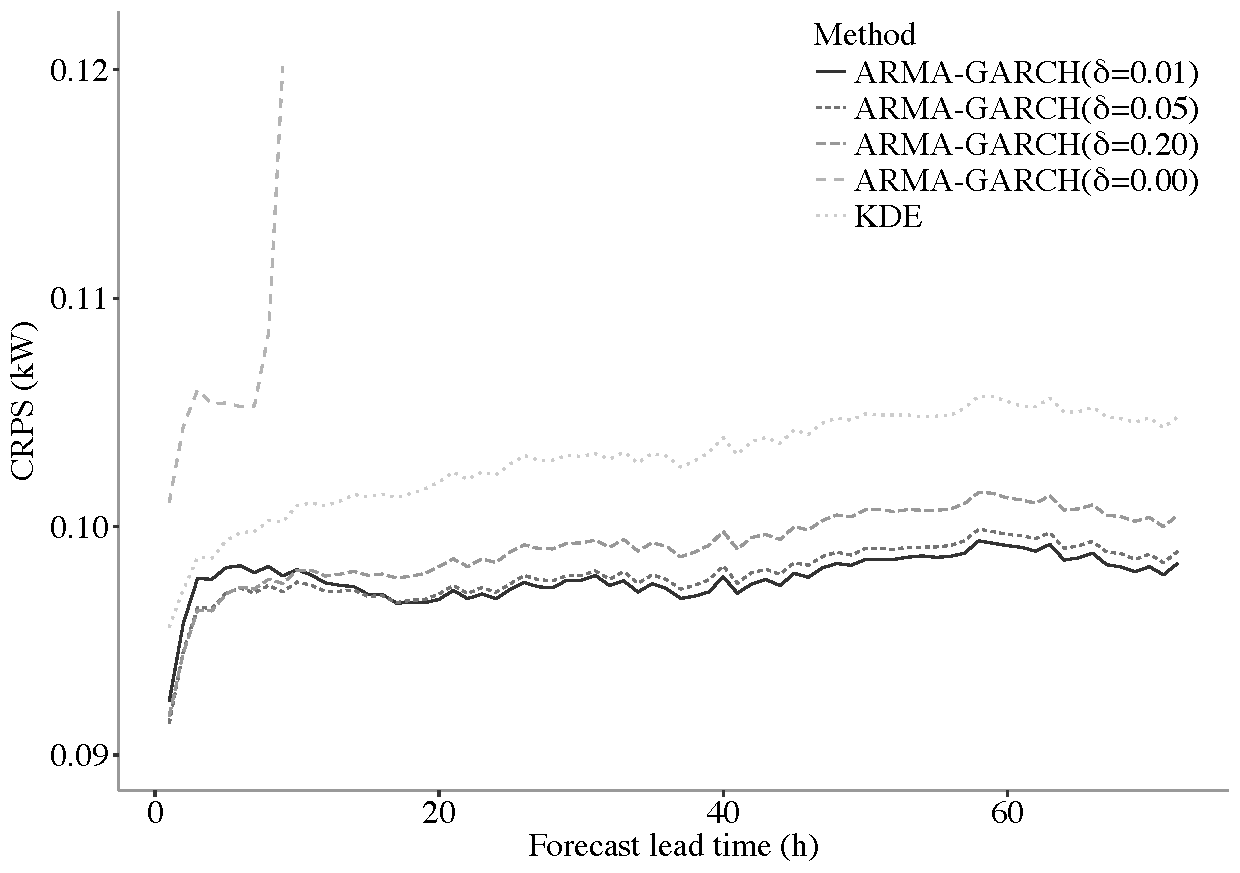
\includegraphics[width=0.8\columnwidth]{2017-10-13_big-gofmin_266_graylinesman.pdf}
  \caption{Goodness-of-fit selection}
  \label{fig:benchmark}
\end{figure}

For this particular dataset, when forecasting for lead times smaller than 12 hours, the ARMA-GARCH ($\delta = 0.05$) model is the best performer.
This model starts to underperform, compared to ARMA-GARCH ($\delta = 0.01$), at some point between lead times of 12 and 18 hours.


%===========================================
\section{Methods for demand aggregation}
\label{sec:load_aggr}
%===========================================
One of the  actors anticipated in the P2P energy marketplace is the P2P Aggregator. \citet{pouttu2017p2p} mention that the P2P aggregator will deliver, among other services, forecasts for aggregated load and generation, and then, for a given expected generation, optimally procure aggregation of demand by combining multiple customer loads, closely matching generation. The goal of our experiment is to propose a method for this. In the composition of the group, the size of customers could vary from one to hundreds customers.

In order to understand the relationship between demand aggregation and forecast uncertainty, we created several groups containing a random selection of households, within a population of 200 households.
Figure \ref{fig:4weeksaggr} exemplifies how aggregating the demand of several customer reduces the instability of demand.
\hl{mention the period from xx/xx to xx/xx, on x-axis put dates}

\begin{figure}
  \centering
  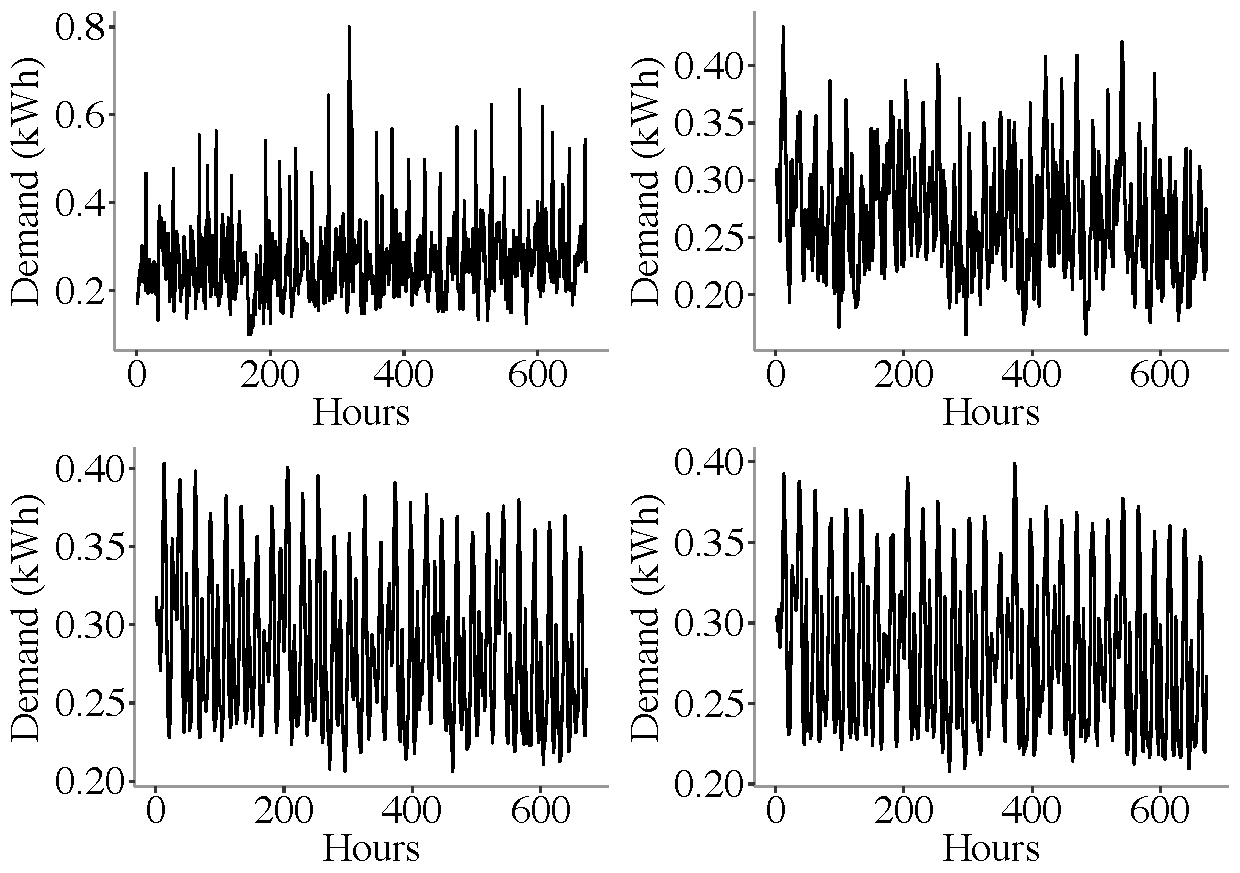
\includegraphics[width=0.8\columnwidth]{2017-10-13_compare_aggrdemands}
  \caption{Example of demand time-series for one customer (top-left), and aggregated demand time-series for ten (top-right), one hundred (bottom-left) and two hundred (bottom-right) customers during a period of four weeks}
  \label{fig:4weeksaggr}
\end{figure}

Each of these groups had their demand forecasted and evaluated through the procedure described on Section \ref{ss:fcst}.
In order to maintain proportional comparability, the aggregated demand value of each group is the sum of its households' demand divided by the number of households.

Figure \ref{fig:rndgrp} represents the forecast accuracy versus the forecast lead time.
As expected, forecast error increases (CRPS value) as the lead time increases.
A strong converging pattern can be seen
The inaccuracy has a major decrease from individual households to groups of 10, while decreases marginally when comparing groups of 100 and 200 households.
This suggests that only increasing the number of individuals per group would not be a optimal solution for reducing forecast uncertainty.
Nevertheless, a larger aggregation is always expected to generate forecasts with lower errors.

\begin{figure}
  \centering
  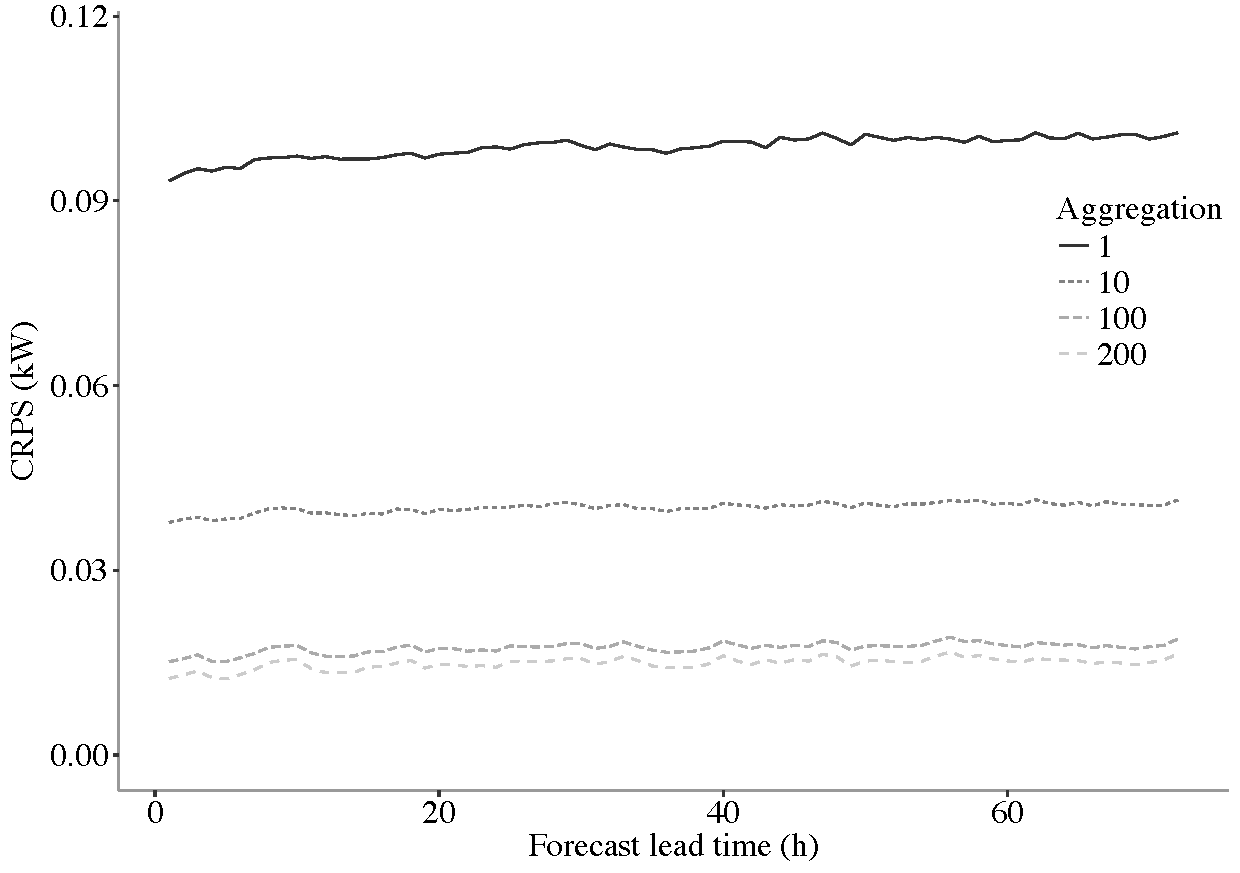
\includegraphics[width=0.8\columnwidth]{2017-10-13_rndgrp}
  \caption{Forecast uncertainty for different sizes of random groups of households for Korean data}
  \label{fig:rndgrp}
\end{figure}

\begin{figure}
  \centering
  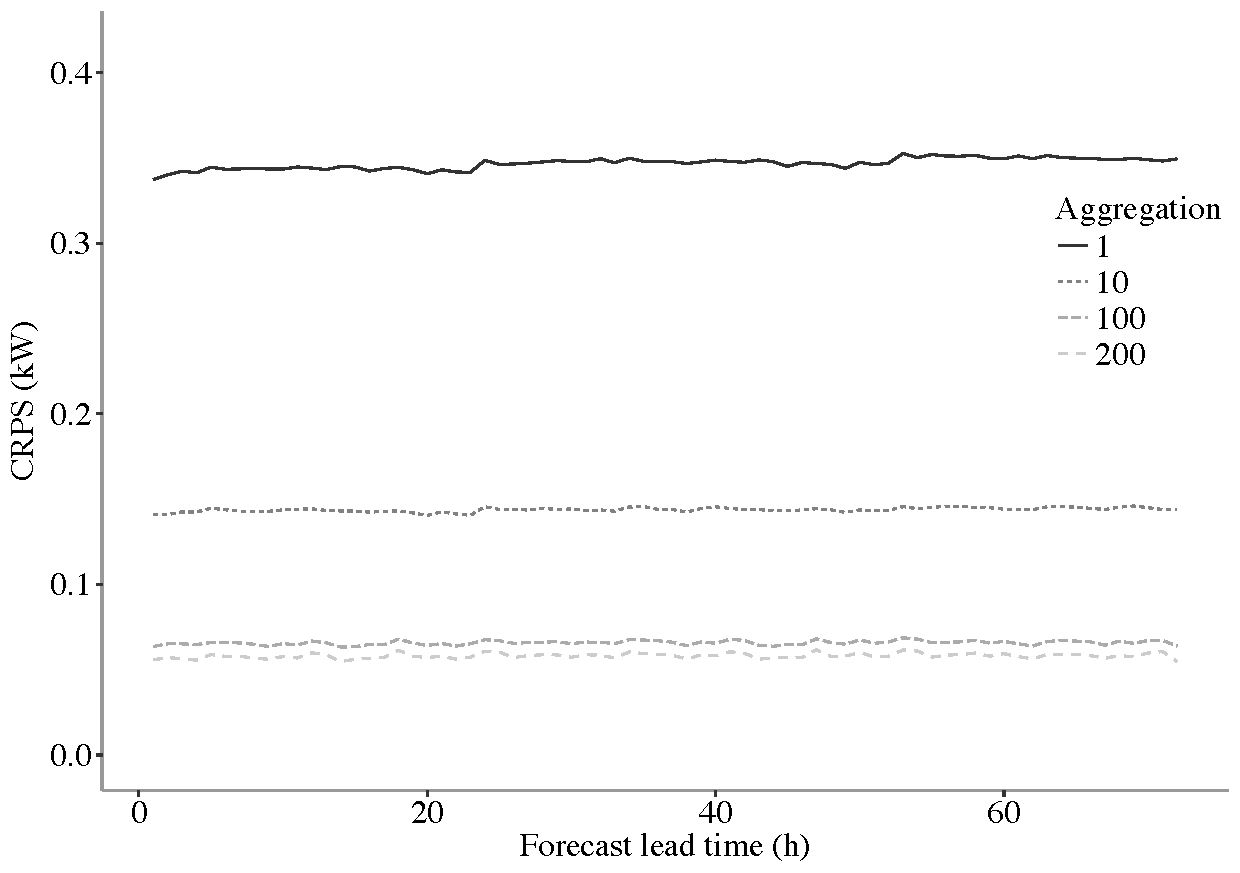
\includegraphics[width=0.8\columnwidth]{2017-12-27_rndgrp_IR}
  \caption{Forecast uncertainty for different sizes of random groups of households for Irish data}
  \label{fig:rndgrpIR}
\end{figure}

This groups created following a random fashion were used every time a portfolio optimisation model was run.
The goal is to visualise where the proposed efficient frontier would seat, comparing to the basic random aggregation.

To select customers, we will consider an efficient frontier on the risk-return relationship, based on the constrained portfolio optimisation algorithm defined in Section \ref{ss:sdevgrp}. We illustrate this in Figure \ref{fig:portoptex}, which relates the average of density forecast errors on the x-axis (risk) to the expected aggregated demand on the y-axis (return). \hl{the selection is random, and then averaged, just to show the pattern}

\begin{figure}
  \centering
  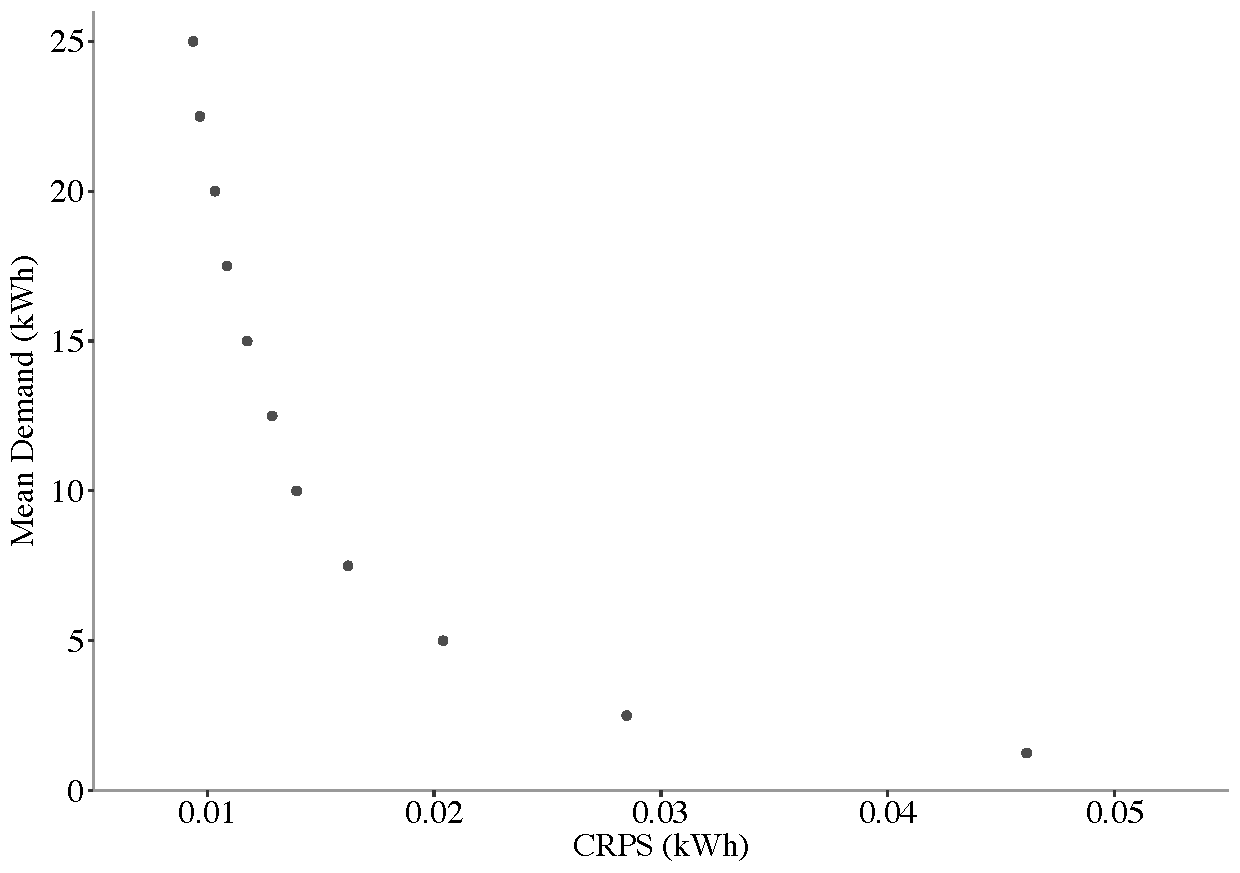
\includegraphics[width=0.8\columnwidth]{2017-11-15_randomgrouping}
  \caption{Example of risk-return frontier for forecast-based energy demand portfolios}
  \label{fig:portoptex}
\end{figure}
\hl{maybe this figure should be on the first pages of the paper?}
Retrieving the expected future aggregated demand for a group of customers is a forecast based task.

On the other hand, minimising the expected forecast error can be performed in many different ways, including forecast based methods.
The Aggregator would use the frontier rendered by different methods to operate in the energy market minimising the risk of under- or over- bidding energy consumption, while trying to match supply offers from distributed energy generation.

\l{review this:} The following pages describe this process. Starting from the seasonality analysis (Section \ref{ss:dtransf}), the forecasting model and evaluation criteria (Section \ref{ss:fcst}), and finally, the portfolio optimisation model (Section \ref{ss:portopt}).

%-------------------------------------------
\subsection{Constrained portfolio optimisation}
\label{ss:sdevgrp}
%-------------------------------------------
Markowitz’s portfolio selection approach studies how investors can construct optimal portfolios, taking into consideration the trade-off between market volatility and expected returns.
For a particular universe of assets, portfolios on the efficient frontier offer the maximum possible expected return for a given level of risk.
One of the several formulations involves the construction of a portfolio with minimal risk provided that a prescribed return level is attained \citep{bonami2009portopt}.
In the P2P energy marketplace scenario, risk and return can, respectively, be interpreted as the expected forecast error of each group of customers and expected aggregated demand.
To construct the efficient frontier in this scenario we need to select groups that, for a given expected aggregated demand returns the lowest expected forecast error.

Classic portfolio optimisation assumes that asset returns follow a multivariate normal distribution.
This means that the return on a portfolio of assets can be completely described by the expected return and the variance.
The portfolios on the efficient frontier can be found by quadratic programming, a widely available and efficient solver.
The solutions are optimal and the selection process can be constrained by practical considerations which can be written as linear constraints \citep{CHANG20001271}.

However, energy demand for different portfolio of customers' demand does not behave like assets for a few reasons:
\begin{enumerate}
   \item The perishable nature of electricity demand;
   \item Restrictions, as customers either participate to a group or not and;
   \item Nonlinear relationship between customer selection and forecast error.
\end{enumerate}

The constrained portfolio optimisation is an extension to the standard model that includes constraints that limit a portfolio to a specified number of assets and impose limits on proportions on selected assets.
\citet{CHANG20001271} present three algorithms based upon genetic algorithms, tabu search and simulated annealing for finding the constrained efficient frontier.
The attraction of these algorithms are the effectively independency of the selected objective function, facilitating the assessment of different non-linear functions.

The properties of this portfolio optimisation extension, coupled with a solution that is valid for a given forecast lead time, would satisfy the unique characteristics of a portfolio of customers' demand, enabling the implementation of a forecast-based portfolio optimisation platform for P2P energy markets.

%-------------------------------------------
\subsection{Forecast-based Portfolio Optimisation}
\label{ss:portopt}
%-------------------------------------------

The constrained portfolio optimisation goal is to find, from possible groups of customers, smaller groups that would deliver high forecasting accuracy.
The constrain is defined as a binary variable where each customer is included or not in a given portfolio.

We chose three different objective functions on our work, further detailed in this Section:
\begin{enumerate}
   \item Forecast Validated (FV): minimising forecast error using the forecasting function on a validation dataset.
   \item Seasonal Residual (SR): minimising standard deviation of the residual of a deseasonalised aggregated demand and;
   \item Seasonal Similarity (SS): minimising the deviation of the seasonal signals of customers pertaining a portfolio;
\end{enumerate}
All three implemented objective functions require a nonlinear function $f_i$.
This function is applied to a matrix $\bm{A}$ containing the demand history (columns) per customer (rows) and a customer selection vector $v$.
Considering restrictions, $v$ was defined as a binary vector with as many positions as the number of households (equation \ref{eq:nonlfx}).
\begin{equation}
   \underset{v_j \in \mathbb N[0,1]}{min}\big(f_i(A,v)\big)
   \label{eq:nonlfx}
\end{equation}
To perform this minimisation, we chose a genetic algorithm approach as this have been proven to perform marginally better than tabu search and simulated annealing for constrained portfolio optimisation problems \citep{CHANG20001271}.
We used the pure genetic algorithm option with R function \texttt{\textbf{genoud}} disabling the derivative information option \citep{rgenoud}.
\texttt{\textbf{genoud}} uses a generation based optimisation, modifying a population of trial solutions so each generation is expected to be better than its predecessor, measured against the function to be optimised.
This algorithm also allows for integer constraints to be implemented on the variable space, outside the objective functions, which dramatically reduces computational time.

Using derivatives is not mandatory, but in some cases might speed up the convergence on local optima.
However, optimisation methods that rely on derivatives of the objective function may be unable to find optimum values when dealing with nonlinear functions and integer variables due to non-concavity and discontinuities \citep{genoud}.

Sections \ref{sss:FV} to \ref{sss:SS} describe the three proposed objective functions.
Further, Section \ref{ss:res_demaggr} present the results from different optimisation approaches, followed by discussions on Section \ref{sec:discussion}.

%-------------------------------------------
\subsubsection{Forecast Validated (FV) function}
\label{sss:FV}
%-------------------------------------------
The FV method is the most straight forward of the three selection functions.
The objective is the optimisation of the group selection based on the forecast accuracy.
Specifically, the FV method divides $\bm{A}$ into a training matrix $\bm{A_a}$ and a test matrix $\bm{A_b}$.
A density forecast $g$ is then produced using the training matrix, while the evaluation occurs against the test matrix.
\begin{equation}
   F_{fv}\big(g(\bm{A_a} \times v),\bm{A_b} \times v \big)
   \label{eq:fv}
\end{equation}

$F_{fv}$ returns the forecast accuracy of the evaluation step.
The goal of the optimiser is the minimisation of Equation \ref{eq:fv}, through changing $v$.
The vector $v$ that delivers the minimal value of $F_{fv}$ is the customer selection that minimises the forecast error through the FV function.

For setting up the FV function, we divided $\bm{A}$ into $n=16$ partitions to enable multiple runs in a rolling forecast fashion.
This allowed the forecast evaluation of several positions in the in-sample dataset against the same selection vector $v$.
This number of divisions rendered a good trade-off between optimisation result, over-fitting, and computational time.

$F_{fv}$ was applied to each training matrix $\bm{A}_{n,a}$ and evaluated against the test matrix $\bm{A}_{n,b}$, using the same selection vector $v$.
The average of these evaluations was returned as the FV function result, and as described in Section \ref{sss:FV}, $v$ was chosen in order to minimise this result.
An alternative approach, that selected only the last day instead of the last week of the in-sample period, was implemented as well, rendering less accurate forecasts through the chosen selection vector $v$ (see Table \ref{tb_fvperselec}).

\begin{table}[]
	\centering
	\caption{Results for different in-sample period oversaw by FV optimisation}
	\label{tb_fvperselec}
	\begin{tabular}{@{}ll@{}}
	\toprule
	\multicolumn{1}{c}{\textbf{\begin{tabular}[c]{@{}c@{}}In-sample period\end{tabular}}} & \multicolumn{1}{c}{\textbf{Average CRPS}} \\ \midrule
	1 day                                                                                                             & 0.006921313                               	\\
	7 days                                                                                                            & 0.006198084                               	\\ \bottomrule
	\end{tabular}
\end{table}

%-------------------------------------------
\subsubsection{Seasonal Residual (SR)}
\label{sss:SR}
%-------------------------------------------
The SR method aggregates the time-series data of a defined group of customers, followed by the seasonality analysis.
The seasonality analysis returns the remainder signal of the seasonal decomposition from the aggregated demand history.
Finally it calculates the standard deviation of this single time-series data containing to the remainder of the decomposition.

On other words, applies the following $F_{sr}$ function onto the undivided matrix $\bm{A}$ and the selection vector $v$, as shown in equation \ref{eq:sr}.

\begin{equation}
   F_{sr}(\bm{A},v) = \widehat{RSD}(R^{\bm{A} \times v}_t)
   \label{eq:sr}
\end{equation}

Where:

$\widehat{RSD}$ is given by the sample standard deviation $s$ divided by the mean $\bar{x}$;

$R^{\bm{A} \times v}_t$ is defined as the remainder of the seasonal decomposition (described on Section \ref{ss:dtransf}) onto the time-series generated after multiplying matrix $\bm{A}$ with the selection vector $v$, as in equation \ref{eq:stlsr}.

\begin{equation}
   STL (\bm{A} \times v)_t = T^{\bm{A} \times v}_t + S^{\bm{A} \times v}_t + R^{\bm{A} \times v}_t
   \label{eq:stlsr}
\end{equation}

The goal of the optimiser is the minimisation of the SR function $F_{sr}$ applied to $\bm{A}$, through changing $v$.

%-------------------------------------------
\subsubsection{Seasonal Similarity (SS)}
\label{sss:SS}
%-------------------------------------------
The SS method is a bi-objective optimisation using function $F_{ss}$ applied onto the undivided matrix $\bm{A}$ through the selection vector $v$, using the objective ratio $r$.
While both FV and SR use $v$ to multiply $\bm{A}$ and generate a single time series to be used by the optimisation, SS uses $v$ to create a new demand history matrix $B$ that is a partition of $\bm{A}$, and includes only the rows of selected customers.

The function then performs a seasonal decomposition on each row $i$ of $B$, following equation \ref{eq:stlss}.

\begin{equation}
   STL (\bm{B_t}) = \bm{T^B_t} + \bm{S^B_t} + \bm{R^B_t}
   \label{eq:stlss}
\end{equation}

Matrix $\bm{S^B_t}$ contains the seasonal component for each customer, while matrix $\bm{R^B_t}$ contains the remainder of the seasonal decomposition for each customer.
The bi-objective approach estimates the relative standard deviation ($\widehat{RSD}$) per column and then averages the result per matrix, before applying the bi-objective ratio $r$.

\begin{equation}
   F_{ss}(\bm{A},v,r) = \frac{\sum_{j=1}^{n}\widehat{RSD}({\bm{S^B_t}}_j)}{n} (r) + \frac{\sum_{j=1}^{n}\widehat{RSD}({\bm{R^B_t}}_j)}{n} (1-r)
   \label{eq:ss}
\end{equation}

Where $\widehat{RSD}$ is given by the sample standard deviation $s$ divided by the mean $\bar{x}$.

The first part of Equation \ref{eq:ss} calculates the similarity between the seasonal components of selected customers. Lower $\widehat{RSD}(\bm{S^B_t})$ per column means minimal difference between seasonal signals per time-step. The second part of Equation \ref{eq:ss} calculates the similarity between the remainder components of selected customers. Since it is expected that $\bm{R^B_t}$ has no trend, a second consequence is that lower $\widehat{RSD}(\bm{R^B_t})$ means customers with lower variability after removing the seasonal signal. Different ratio $r$ can be used to change the weights between the objective functions.

The goal of the optimiser is the minimisation of Equation \ref{eq:ss}, through changing $v$ for a given $r$.

For setting up the SS function, three groups of options were explored on the process described on Section \ref{sss:SS}.
\begin{enumerate}
	\item prior execution of a normalisation routine on component $S^B_t$ before comparing the similarity of the seasonal behaviour;
	\item either focusing the similarity comparison on the selected forecast lead time of $S^B_t$ or on the entire seasonal component;
	\item changing the weights for the bi-objective function
\end{enumerate}
The different results on forecast accuracy for each combination of options $1$ and $2$ are presented on Table \ref{tb_ssmix_nf}.
The non-normalisation of seasonal component while considering the entire in-sample dataset, instead of focusing on the forecast lead time, rendered the best result for Korean data.

\begin{table}[]
	\centering
	\caption{Results for SS function running with different configuration on prior normalisation routine and forecast lead-time focus for similarity evaluation}
	\label{tb_ssmix_nf}
	\begin{tabular}{@{}ll@{}}
	\toprule
	\multicolumn{1}{c}{\textbf{\begin{tabular}[c]{@{}c@{}}Configuration\end{tabular}}} & \multicolumn{1}{c}{\textbf{Average CRPS}} \\ \midrule
	Non-normalised and focused                                                                                     & 0.008493832                               	\\
	Normalised and focused                                                                                         & 0.008264960
	\\
	Non-normalised and non-focused																				   & 0.006933789
	\\
	Normalised and non-focused																				       & 0.008999768
	\\ \bottomrule
	\end{tabular}
\end{table}

Having selected the first two options, the different weights were assessed and Table \ref{tb_ssmix_r} summarises the findings.
For the same dataset, giving a weight  $r = 0.1$ to the seasonal component, while ignoring the remainder similarity on the bi-objective function, returned the best accuracy.

\begin{table}[]
	\centering
	\caption{Results for SS function running with different configuration on weights given to bi-objective function}
	\label{tb_ssmix_r}
	\begin{tabular}{@{}ll@{}}
	\toprule
	\multicolumn{1}{c}{\textbf{\begin{tabular}[c]{@{}c@{}}Configuration\end{tabular}}} & \multicolumn{1}{c}{\textbf{Average CRPS}} \\ \midrule
	Seasonal component given weight 1.0                                                                            & 0.007203195                               	\\
	Seasonal component given weight 0.8                                                                            & 0.008410930                               	\\
	Seasonal component given weight 0.5                                                                            & 0.007606566                               	\\ \bottomrule
	\end{tabular}
\end{table}

%-------------------------------------------
\subsection{Genetic algorithm optimisation}
\label{ss:genoud}
%-------------------------------------------

The genetic algorithm was set to stop after $100$ generations or after $10$ consecutive generations without enhancement in the function value, whatever happened first.
For all methods, we used 12 weeks as the in-sample period (matrix $\bm{A}$, containing 100 customers as rows, and 2016 time-steps as columns).
Instead of running the optimisation to find one unique optimal group, we divided the expected demand axis into $16$ bins.
This method was chosen to enable the construction of a stepwise efficiency frontier for each optimisation function.
Practically this means that, for any chosen function, instead of running a single optimisation run on $\bm{A}$ for the full spectrum of expected demand, we run $16$ optimisations with different and non-super-positioned expected demand limits.
The process created groups whose aggregated demand would be between given minimum and maximum values.
This number of divisions was selected as they enabled the construction of a piecewise frontier while allowing the entire process to be executed in a feasible computational time.

%-------------------------------------------
\subsection{Results for demand aggregation}
\label{ss:res_demaggr}
%-------------------------------------------
\hl{explain the 100 sims plot}


%===========================================
\section{Discusion}
\label{sec:discussion}
%===========================================

%-------------------------------------------
\subsection{Portfolio optimisation results for Korean data}
\label{ss:portoptKO}
%-------------------------------------------
Figures \ref{fig:optKO_04h} and \ref{fig:optKO_12h} present the portfolio optimisation for two different time-ahead forecasts. This results are the average values from 11 different simulations, each containing 100 customers from the Korean dataset.
Table \ref{tb_optKO} summarises the results, averaging the accuracy value throughout the energy demand spectrum for all functions.
All three optimisation functions implemented deliver good result at selecting groups that would reduce the uncertainty for given mean demand ranges.
As the mean demand increases, a simple random aggregation of customers are able to reduce most of the uncertainty, leaving a limited space for optimisation (upper part of the figures).
Nevertheless the portfolio optimisation returns the best available groups (or very close to it) most of the time, specially for the SS and FV functions.
On both forecast lead-times the SS functions perform poorly compared to the alternatives.
Also, one can see that a longer forecast lead-time render a worse accuracy for random groups of customers.

\begin{figure}
  \centering
  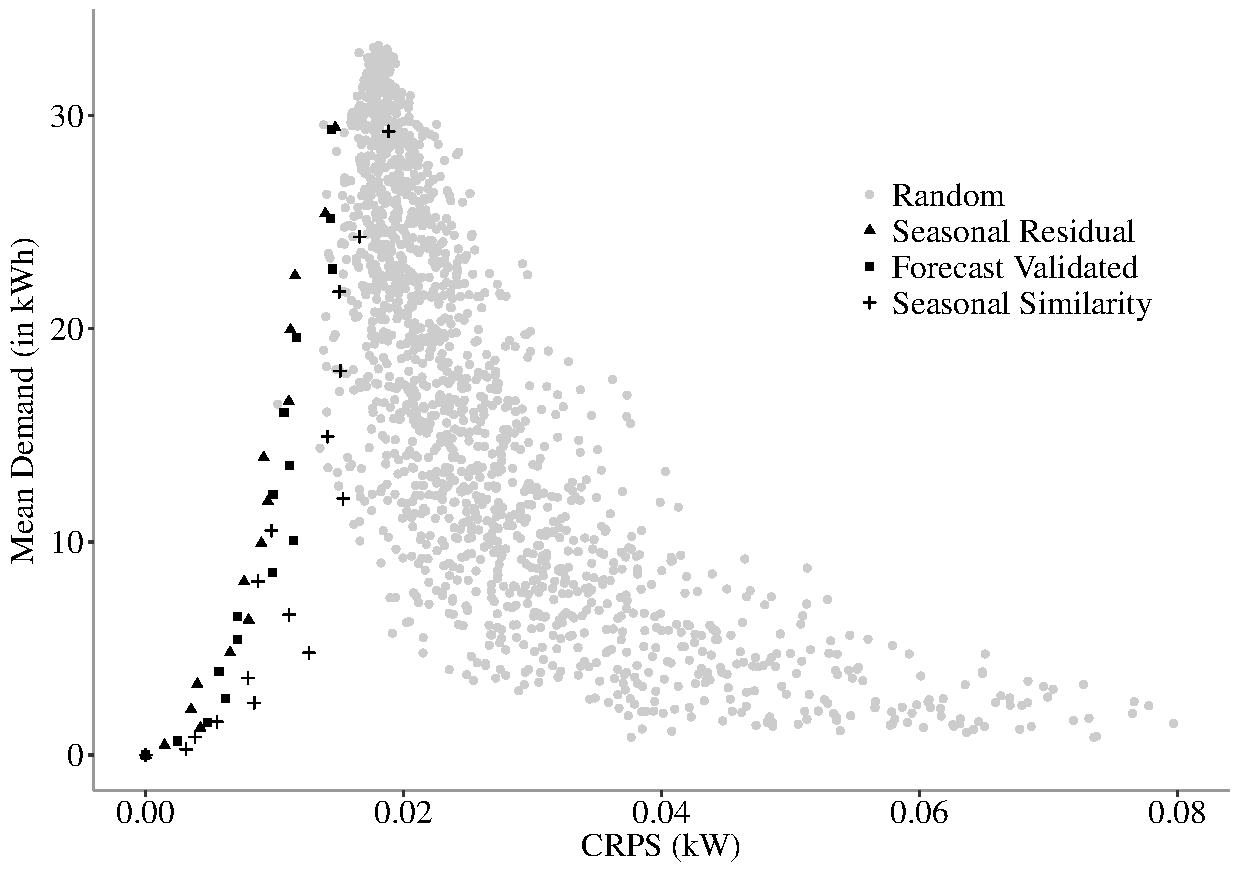
\includegraphics[width=0.8\columnwidth]{2017-11-27_runf_KO_04h.pdf}
  \caption{Portfolio optimisation using a 4h-ahead forecast for Korean customers}
  \label{fig:optKO_04h}
\end{figure}

\begin{figure}
  \centering
  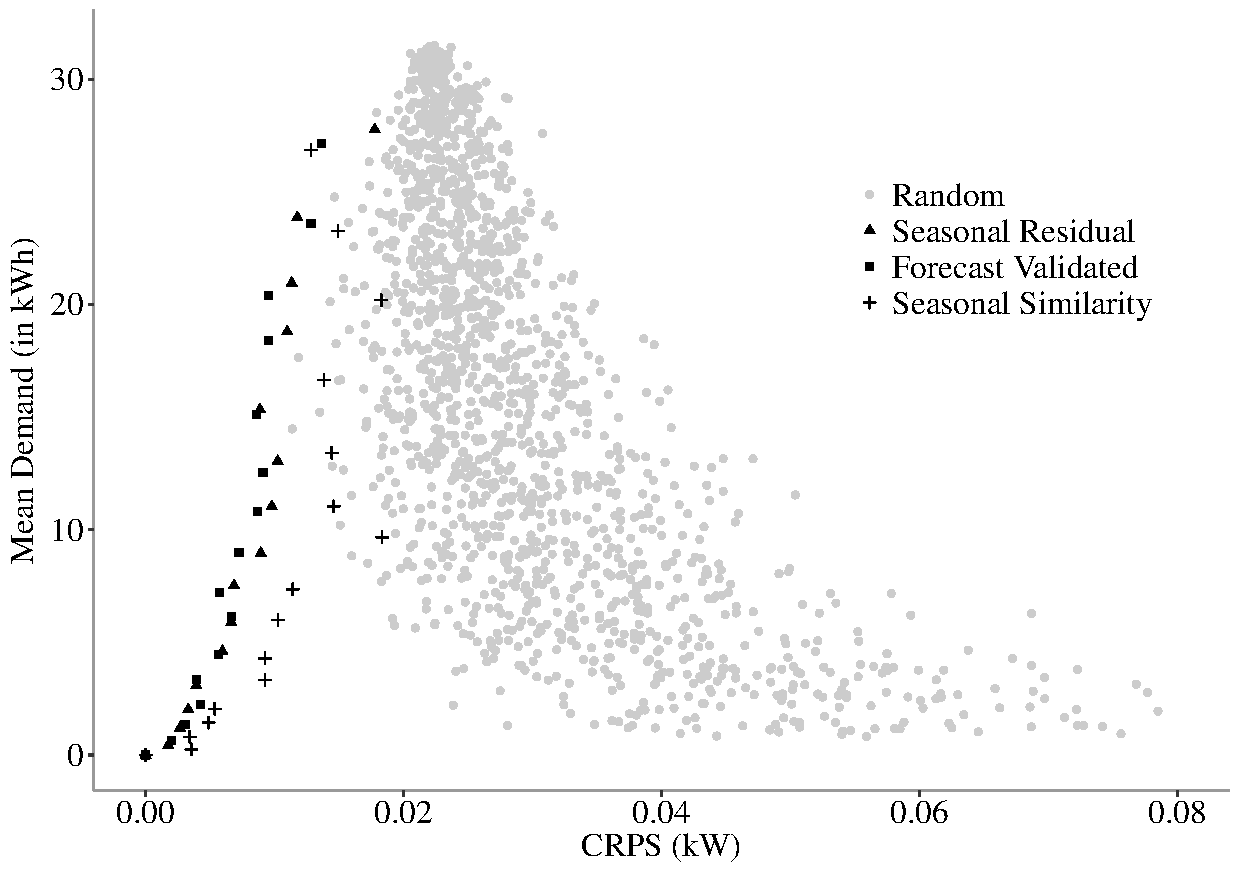
\includegraphics[width=0.8\columnwidth]{2017-11-27_runf_KO_12h.pdf}
  \caption{Portfolio optimisation using a 12h-ahead forecast for Korean customers}
  \label{fig:optKO_12h}
\end{figure}

\begin{table}[]
	\centering
	\caption{Average portfolio optimisation results for different functions and lead-times, using Korean data}
	\label{tb_optKO}
    \begin{tabular}{@{}cll@{}}
    \toprule
    \textbf{\begin{tabular}[c]{@{}c@{}}Optimisation\\ Function\end{tabular}} & \multicolumn{1}{c}{\textbf{\begin{tabular}[c]{@{}c@{}}Average CRPS\\ 4h-ahead\end{tabular}}} & \multicolumn{1}{c}{\textbf{\begin{tabular}[c]{@{}c@{}}Average CRPS\\ 12h-ahead\end{tabular}}} \\ \midrule
	Random                                      & 0.026942760       & 0.029939163                        	\\
	Seasonal Residual                           & 0.007866620       & 0.007564032                        	\\
	Forecast Validated                          & 0.008857013       & 0.006906969                        	\\
	Seasonal Similarity                         & 0.010399700       & 0.010303772                       	\\ \bottomrule
	\end{tabular}
\end{table}

%-------------------------------------------
\subsection{Portfolio optimisation with the Irish data}
\label{ss:portoptIR}
%-------------------------------------------
\hl{Comparison of the two data sets}

In addition, we run the same SR function using the Irish dataset.
The results are still good to generate groups on the lower half of the aggregated demand, but not overcoming as good as the number of customers needed for grouping increases.
Specially for very large aggregations, this method produces groups that are worse than the average of a random grouping method.

\begin{figure}
  \centering
  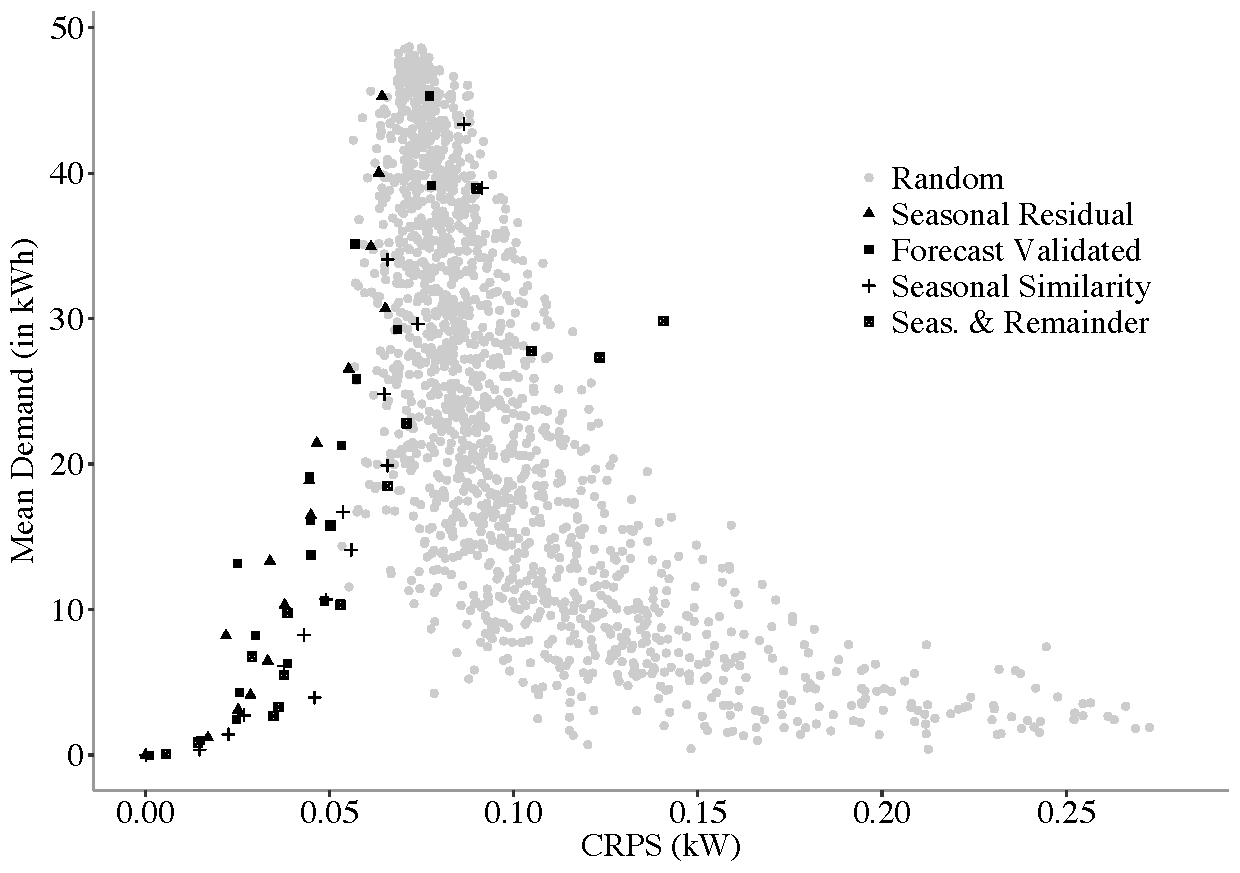
\includegraphics[width=0.8\columnwidth]{2017-12-27_runf_IR_12h.pdf}
  \caption{Portfolio optimisation using a 12h-ahead forecast for Irish customers}
  \label{fig:optIR_12h}
\end{figure}

\begin{figure}
  \centering
  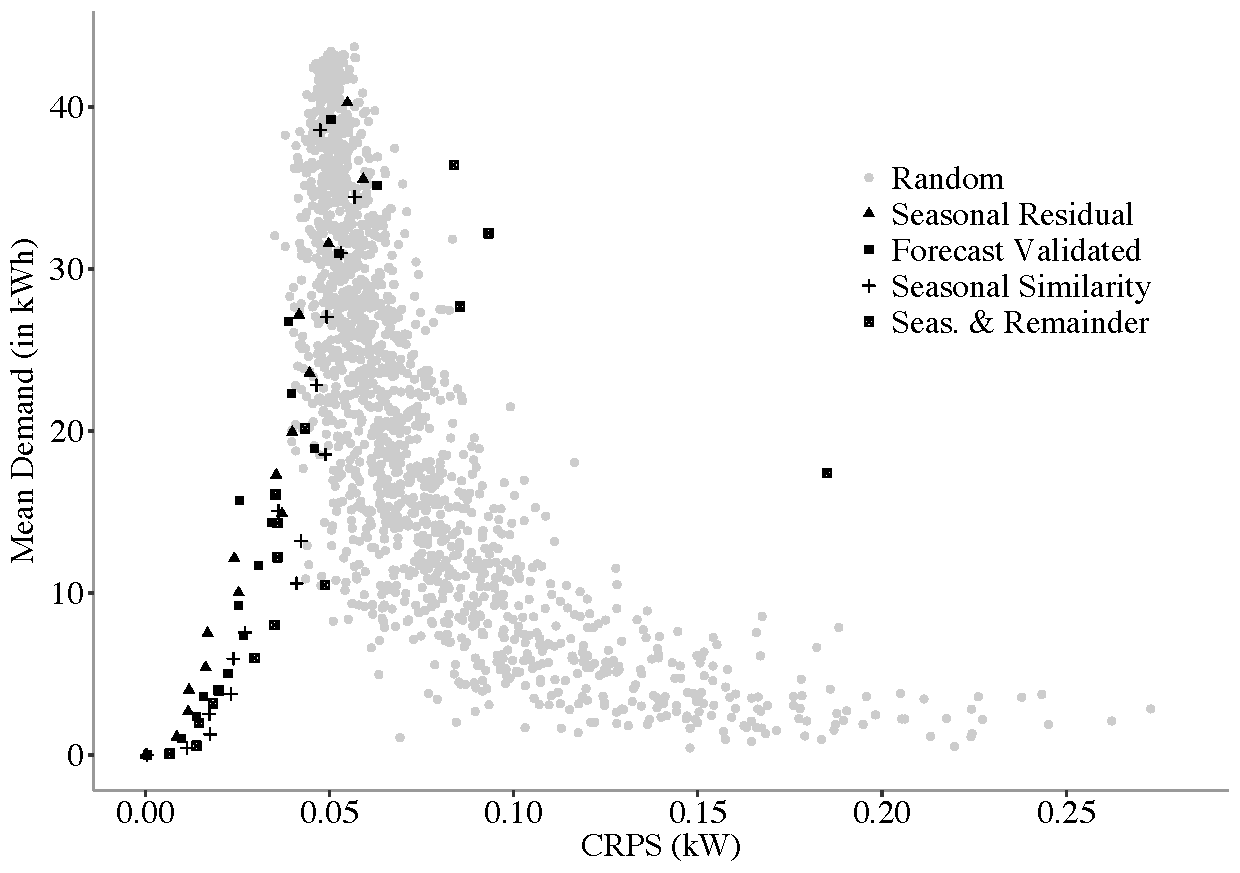
\includegraphics[width=0.8\columnwidth]{2017-12-27_runf_IR_04h.pdf}
  \caption{Portfolio optimisation using a 4h-ahead forecast for Irish customers}
  \label{fig:optIR_04h}
\end{figure}

\begin{figure}
  \centering
  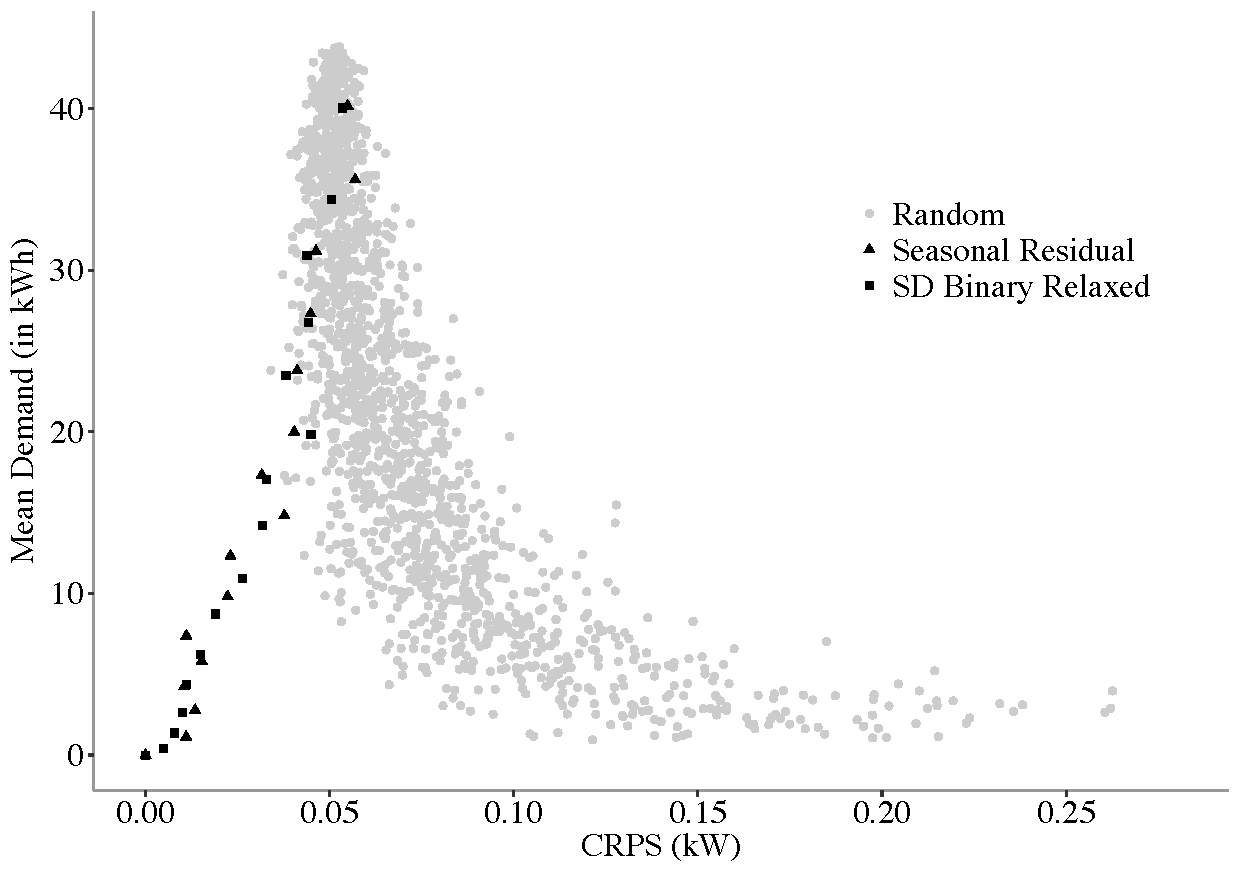
\includegraphics[width=0.8\columnwidth]{2017-12-27_runf_IR_04h-rlx.pdf}
  \caption{Portfolio optimisation using a 04h-ahead forecast for Irish customers, relaxing the binary variable}
  \label{fig:optIR_04h-rlx}
\end{figure}


%-------------------------------------------
\subsection{Comparison between SR and FV functions}
\label{ss:SRxFV}
%-------------------------------------------
The Seasonal Residual (SR) function assumes the same group regardless of the forecast lead time, selecting customers with a high likelihood of minimal standard deviation from a deterministic seasonal decomposition, based on history demand.
On the other hand, the Forecast Validated (FV) approach allows us to find the optimal composition of households on a certain forecast lead time of our interest.
In respect to that, a group created for a $t_{f1} = 4$ forecast might not be the best grouping for a $t_{f2} = 24$.

Another characteristic of the FV method is that it allows groups of customers with high variance aggregated remainder signal to be included, as long as their forecast is stable throughout the training dataset.
This can be seen as an advantage, as it increases the opportunities for grouping, and as an disadvantage as well, as it enables groups with unforeseen inaccurate forecasts to be created.
Another drawback of this functions is the presence of overfitting as groups can be created perfectly when looking at the training dataset, while their performance on the test dataset does not hold.
In someway, the advantages and disadvantages seem to compensate each other, as the FV function performs slightly better for a longer lead-time, and slightly worse for the short lead-time.

Computationally speaking, any signal analysis method (SR or SS) consumes significantly lower time to run as they do not require many forecasting runs while grouping customers.
The FV function needs thousands of forecast runs while grouping, and this can get very time intensive.
On our experiments, with our subset of data and a 2016 8-core i7 processor, FV optimisation costs 27h to build an entire frontier for a single simulation, while the SD function runs ins less than 1h.

%-------------------------------------------
\subsection{Relaxing the binary constraint}
\label{ss:rlx}
%-------------------------------------------
In order to assess if a relaxation of the binary constraint would produce different results, we chose to implement a SR function allowing fractions of each household to be selected for grouping (figure \ref{fig:optKO_04h-rlx}).
It can be seen as there is not much advantage in allowing this selective grouping, with both relaxed and unrelaxed versions of SR performing similarly.

\begin{figure}
  \centering
  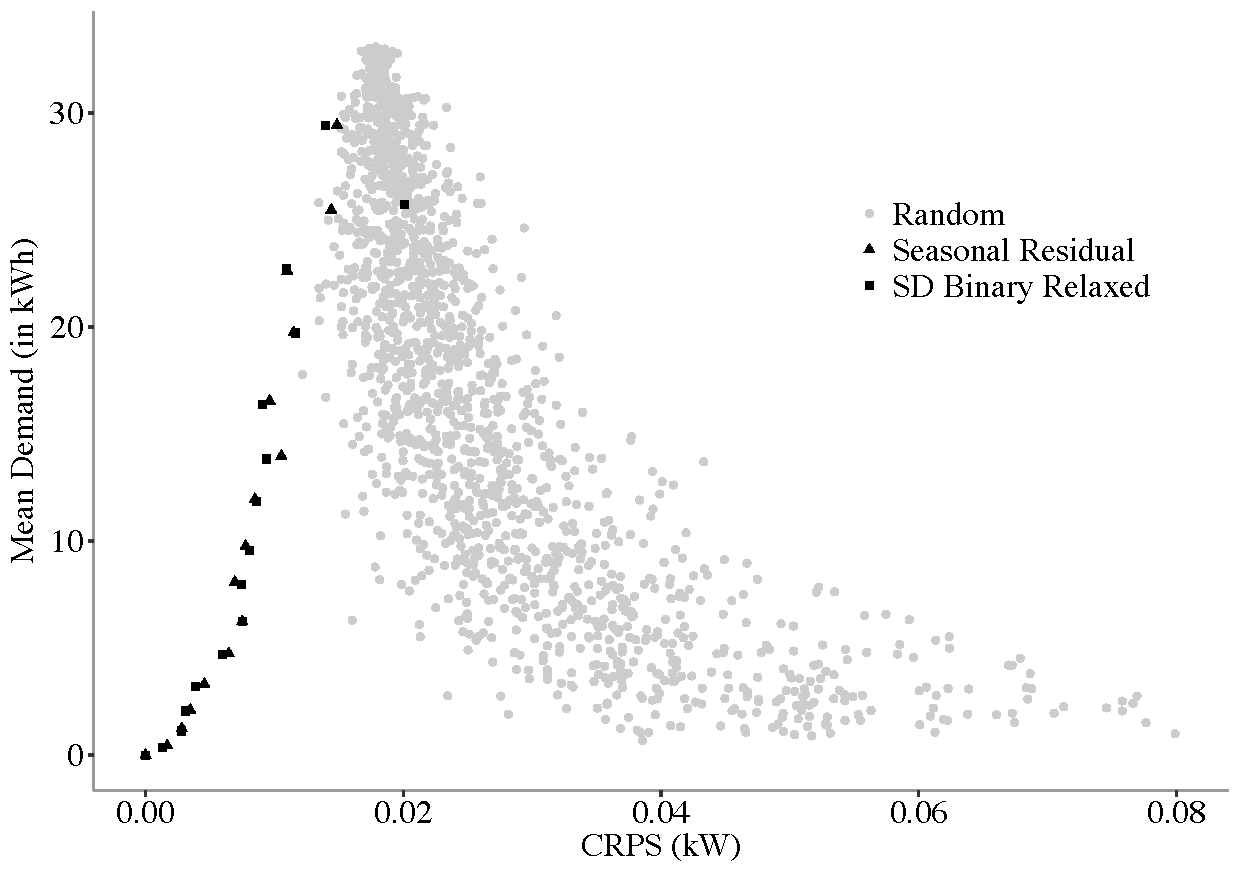
\includegraphics[width=0.8\columnwidth]{2017-11-27_runf_KO_04h-rlx.pdf}
  \caption{Portfolio optimisation relaxing the binary constraint on the 4h-ahead forecast for Korean customers}
  \label{fig:optKO_04h-rlx}
\end{figure}



%===========================================
\section{Conclusion}
\label{sec:conclusion}
%===========================================

\section*{References}

%% The Appendices part is started with the command \appendix;
%% appendix sections are then done as normal sections
%% \appendix

%% \section{}
%% \label{}

%% References
%%
%% Following citation commands can be used in the body text:
%% Usage of \cite is as follows:
%%   \cite{key}          ==>>  [#]
%%   \cite[chap. 2]{key} ==>>  [#, chap. 2]
%%   \citet{key}         ==>>  Author [#]

%% References with bibTeX database:

\bibliographystyle{elsarticle-harv}
\bibliography{mainbib_copy}

%% Authors are advised to submit their bibtex database files. They are
%% requested to list a bibtex style file in the manuscript if they do
%% not want to use model1-num-names.bst.

%% References without bibTeX database:

% \begin{thebibliography}{00}

%% \bibitem must have the following form:
%%   \bibitem{key}...
%%

% \bibitem{}

% \end{thebibliography}


\end{document}

%%
%% End of file `elsarticle-template-1-num.tex'.
